\documentclass[convert = false, tikz]{standalone}
\usepackage[utf8]{inputenc}
\usepackage{tikz}
\usepackage{adjustbox}
\usetikzlibrary{automata, positioning, arrows, fit}
 
% arara: pdflatex
% arara: latexmk: { clean: partial }
\begin{document}
    \tikzset{
    every state/.style={draw=none, text centered, align=center, inner sep=1mm}, % sets style for all states
    }
    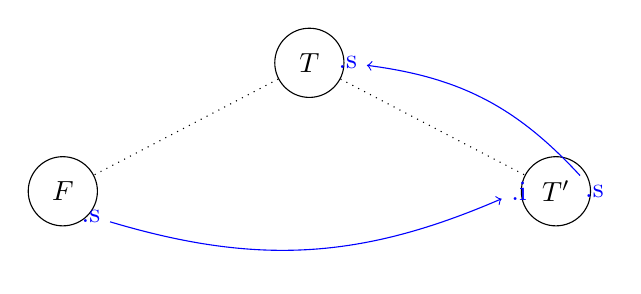
\begin{tikzpicture}[node distance=1cm and 2.5cm]
        % First level
        \node[state] (a) {$T$};

        % Second level
        \node[state, below left = of a] (b) {$F$};
        \node[state, below right = of a] (c) {$T'$};

        % Dotted edges
        \draw 
        (a) edge[dotted,-] node{} (b) % from 1st level to 2nd level
        (a) edge[dotted,-] node{} (c);

        % Blue nodes
        \node[right=0mm of a, xshift=-2mm, align=center, blue] (a_s) {.s};
        \node[below right=0mm and 0mm of b, yshift=2mm, xshift=-2mm, align=center, blue] (b_s) {.s};
        \node[right=0mm of c, xshift=-2mm, align=center, blue] (c_s) {.s};
        \node[left=0mm of c, xshift=2mm, align=center, blue] (c_i) {.i};
        
        % Blue arrows
        \draw
        (b_s) edge[->, blue, bend right = 20] node{} (c_i) 
        (c_s) edge[->, blue, bend right = 20] node{} (a_s);

    \end{tikzpicture}
\end{document}